\chapter{Projektbeskrivelse}

\section{Projektgennemførelse}
Projektet startede med, at der blev lavet en tidsplan, som var mulig at ændre undervejs, dog med faste deadlines, som skulle overholdes. De forskellige deadlines lagde op til, at der kunne arbejdes efter vandfaldsmodellen, hvilket dette projekt følger, se figur 6.1. Vandfaldsmodellen går ud på, at der først stilles nogle krav til produktet. Derefter designes produktet på papiret, hvor udseende og kunnen beskrives. Efterfølgende implementeres produktet ud fra krav og design. Til slut udføres accepttest, hvor der testes i forhold til de funktionelle og ikke-funktionelle krav, der er stillet til produktet.

\begin{figure}[H]
	\centering
	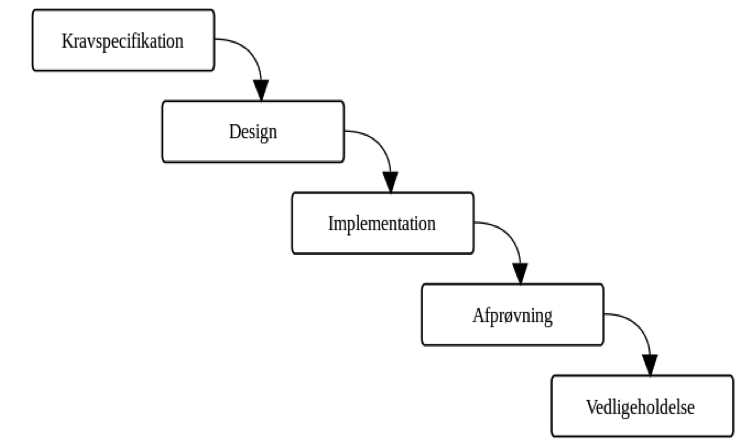
\includegraphics[width=1\textwidth]{Figurer/Snip20150522_15}
	\caption{Vandfaldsmodel}
\end{figure}

Projektgruppen har været på 8 medlemmer, som er blevet delt ind i 2 grupper. Den ene gruppe arbejdede med softwareudviklingen, mens den anden gruppe arbejdede med dokumentation og udarbejdelsen af design. Da gruppen har været opdelt, har der været projektmøde hver uge, hvor gruppen har opdateret hinanden og rettet tidsplanen til, hvis det var nødvendigt.


\section{Metode} 
Dette afsnit har til formål at beskrive hvilke metoder, der er benyttet i udarbejdelsen af projektet. Primært er der tale om metoder fra faget ISE samt Sundhedsvidenskab.\\ 
Desuden bliver der i dette afsnit også beskrevet hvilke arbejdsredskaber, der er benyttet til udførelse af projektet, rapporten og dokumentationen.\\ \\
Til beskrivelse samt opbygning af EKG-systemet er der fra ISE benyttet metoden SysML. SysML er en metode, der vha. digrammer analyserer, specificerer, designer og verificerer et givet system. Altså er metoden benyttet til at beskrive systemets opbygning og kommunikationen. \\ 
Yderligere er der en applikationsmodel, hvor et samlet overblik over systemet er beskrevet. Denne model består af en domænemodel, hvor alle aktiviteterne i systemet er beskrevet samt tilhørende klassediagrammer med metoder fra SD. SD beskriver systemets virkning og hvordan de enkelte dele interagerer, hvilket er specifik for hver enkelt use case.\\ 
Softwaren er beskrevet gennem metoden UML, helt specifikt ved et UML klassediagram. Klassediagrammet viser, hvilke klasser og metoder al softwaren (med undtagelse af blackbox) består af samt, hvordan systemet er bygget op efter trelagsmodellen.\\
Baggrundsafsnittet, afsnit 3, er udarbejdet ved tekstanalyse og kildekritik, ud fra sundhedsvidenskabelige bøger.\\ \\
Af benyttede arbejdsredskaber er der først og fremmest brugt en fælles arbejdsplatform, GitHub. GitHub er en online platform, hvor der er mulighed for at foretage ændringer samtidigt, og gemme i en fælles mappe. Yderligere er der mulighed for en detaljeret versionshistorik.\\
Alle SysML- og UML-diagrammer er udarbejdet i programmet Visio. Koden er skrevet i sproget c\#, i programmet Visual Studio. Visual Studio spiller også sammen med programmet WaveForms generator, i forbindelse med simulering af EKG-signalet. Selve rapporten, mødereferater, logbog og dokumentationen er udformet i tekstprogrammet LaTex. Yderligere er Facebook brugt til mødeindkaldelse og generel kommunikation.



\section{Specifikation og analyse}

\textbf{Forklar hele afsnittet!!}
I udarbejdelsen af analysen var der mange komplikationer. Dette skyldes primært, at atrieflimren ikke nødvendigvis påvirker et EKG-signal på samme måde hver gang.\\ \\
Først var der tiltænkt en analyse, som skulle tage udgangspunkt i definition for atrieflimren, hvor der forekommer 220-300 små udsving/minut på baselinen. Måden hvorpå dette skulle foregå, var ved at tage et gennemsnit \textbf{WHAT, hvad betyder det helt præcis} af baseline, og derefter detektere hvor mange gange der skete en svingning over baseline. Her skulle der så tjekkes, om svingningerne overtrådte en tærskel. Denne tærskel skulle vurderes ud fra den patofysiologiske baggrund for sygdommen. Efter visualisering af reelle målinger, blev denne metode dog afskrevet, da baseline ikke bliver repræsenteret ved en regulær linje i reelle signaler. \\ \\ 
Derefter blev der udtænkt en metode med en dynamisk baseline. Denne metode viste sig meget tideligt i udviklingsprocessen, til ikke at være kompatibel. Den største komplikation ved denne metode var at finde en algoritme, der kunne udelukke de kendte takker, som karakteriserer et EKG-signal. Hvis denne algoritme ikke blev fundet, ville den dynamiske baseline altid ligge et stykke over den reelle baseline, grundet de høje R-takker. \\ \\
De to første metoder blev aldrig færdiggjort, da problemerne opstod efter pseudokoden begyndte at blive udarbejdet. Herefter gik gruppen til vejleder for at finde en alternativ løsning til analysen. Vejleder fik herefter input fra en anden professionel, og kunne derefter hjælpe med at udarbejde en analyse, som virkede.\\ \\
Vejleder kunne oplyse, at atrieflimren har specifikke kendetegn, hvis der bliver analyseret på EKG-signalets amplituder inden for specifikke frekvenser, og det er ud fra denne information, at den endelige analyse blev udarbejdet. 

\section{Arkitektur}
Softwaren er bygget op i henhold til trelagsmodellen, hvor GUI’erne fungerer som programmets brugerinterface, med et login-vindue, et CPR-vindue og et EKG-vindue. Her fungerer EKG-vinduet, som det primære vindue, hvor EKG-signaler kan vises, analyseres og gemmes. Præsentationslaget er yderligere beskrevet i dokumentationen 3.3.1, men kan også visualiseres ud fra figur 6.2 nedenfor.

\begin{figure}[H]
	\centering
	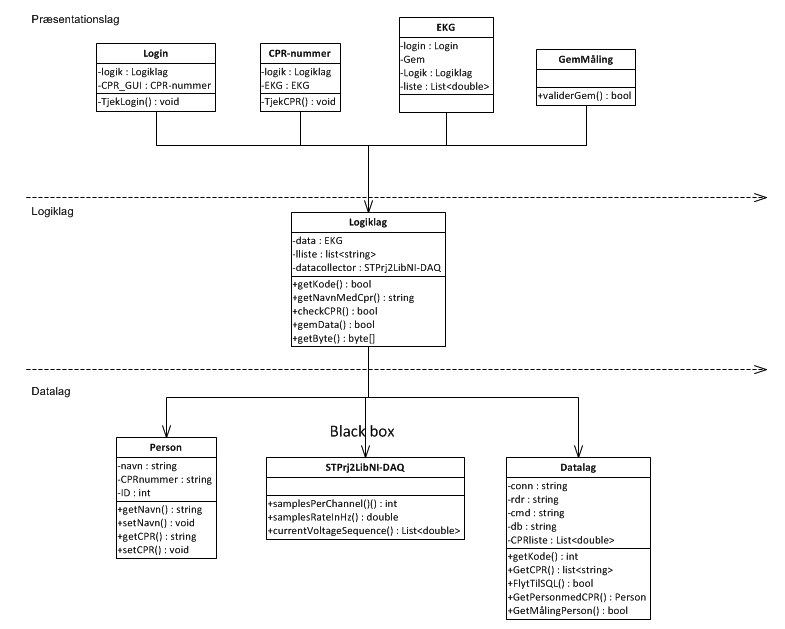
\includegraphics[width=1\textwidth]{Figurer/Snip20150512_9}
	\caption{UML-klassediagram}
\end{figure}
 
Logiklaget kan ses som kernen i softwaren. Det er her alt data bliver behandlet fra datalaget samt videresender data fra målingerne til datalaget. Det er blandt andet her analysen af målingen sker, og hvor indtastede oplysninger bliver valideret. Logiklaget fungerer som bindeleddet mellem de data, der kommer fra datalaget og GUI’erne. \\ \\
Datalaget er til for primært at håndtere forbindelsen til hardwaren og databaserne. I denne klasse bliver der skabt forbindelse til både SQL og DAQ. Datalaget henter data fra den private database, som logiklaget bruger til validering. Denne klasse gemmer også data givet fra logiklaget i både den private- og offentlige database. Klassen "logiklag" og "datalag" er beskrevet yderligere i dokumentationen 3.3.2. \\ \\
For at beskrive koden yderligere, er der lavet en domænemodel. Domænemodellen repræsenterer hele koden, altså hvordan flowet imellem klasserne går, og hvilken overordnet kommunikation, der foregår. Alle vinduerne repræsenterer GUI’er og alle tabeller er tabellerne i den private- og/eller offentlige database. Domænemodellen kan ses på figur 6.3. 

\begin{figure}[H]
	\centering
	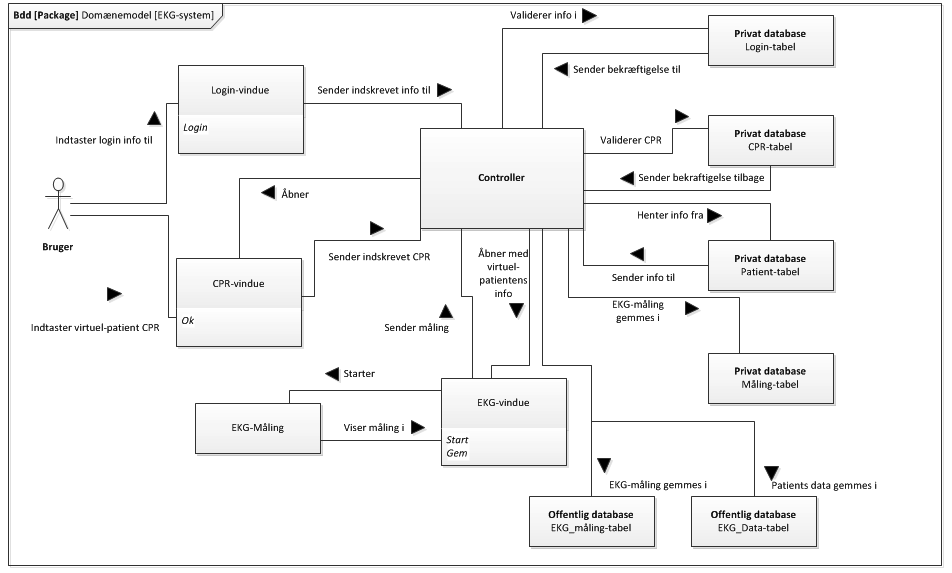
\includegraphics[width=1\textwidth]{Figurer/Snip20150525_18}
	\caption{Domænemodel}
\end{figure}


\subsection{Design}
Alle tanker omkring, hvordan koden skulle være bygget op, bunder i trelagsmodellen. Der er derfor sørget for, at der ikke er noget kode, som kommunikerer med et lag, som de ikke har tilladelse til. Der kan læses mere om trelagsmodellen i dokumentationen 3.3.\\ \\
I dette projekt har der i slutfasen været fokuseret meget på brugervenlighed og feedback til brugeren. Tideligt i projektet var det ikke tydeligt, hvornår der blev foretaget en måling. Dette er blevet tydeliggjort, ved at musen bliver til en cirkel i bevægelse, alt imens der foretages en måling. Der er også lavet et pop-up vindue, som bekræfter, at en måling er blevet gemt.\\ \\
Der er desuden, lavet en feature, som viser grid-lines på grafen. I gruppen blev der besluttet, at der skulle være to typer af grids. En lille og en stor type.  De store grids, repræsenterer hver 0,2 sekunder og de små, svarer til 0,04 sekunder. Disse intervaller er fastlagt, ud fra standarder for professionelle EKG-displays.  Dette blev herefter implementeret i koden.\\ \\
En anden ting, som har været meget dominerende i overvejelserne, er sikkerhed. Da det er personfølsomme oplysninger, som skal detekteres i dette program, er det derfor vigtigt, at det ikke er alle og enhver, som kan få adgang til oplysningerne. Derfor er der et vindue, som beder brugeren om at logge ind, med et gyldigt brugernavn og kodeord. Login-funktionen validere, om denne bruger har rettigheder til at få adgang til systemet.\\ \\
Yderligere er der lavet et patient identifikationsvindue, hvor der skal indtastes et CPR-nummer. Dette CPR-nummer er koblet op til en patient, hvis oplysningen ligger lagret i den private database. Når CPR-nummeret indtastes og EKG-vinduet fremkommer, har programmet været ned i den private database og hentet patienten navn, der stemmer overens med CPR-nummeret. Dette gør det muligt, at få udskrevet navnet i EKG-vinduet. Se eventuelt figur 3.5 i dokumentationen.   

\subsection{Implementering}
Analysen er det essentielle i implementeringen. Hvis ikke der er en analyse, der fungerer, så er programmet obsolet.\\
Analysen er bygget op omkring tre for-løkker, som identificerer forhøjede amplituder inden for et specielt frekvensspektrum. Ved hjælp af matematikbiblioteket alglibnet2, bliver signalet først konverteret til et komplekst Furier-transformeret array, som indeholder koordinater repræsenterende vektorer for amplituden i signalet. Denne konvertering, ses på figur 6.4. \textbf{WHAT, hvad mener du? + figur henvisning} 

\begin{figure}[H]
	\centering
	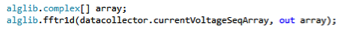
\includegraphics[width=0.8\textwidth]{Figurer/Snip20150525_41}
	\caption{Kode udsnit af analyse implementering}
\end{figure}

Herefter bliver amplituderne regnet ud, ved hjælp af standard formelen for vektorudregning. Disse værdier bliver tilføjet til en ny liste. Dette ses på figur 6.5 nedefor.

\begin{figure}[H]
	\centering
	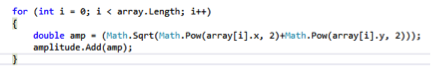
\includegraphics[width=1\textwidth]{Figurer/Snip20150525_43}
	\caption{Kode udsnit af analyse implementering}
\end{figure}

Efterfølgende bliver arrayet udspecificeret til kun, at indeholde de pladser, som repræsenterer amplituderne for det valgte frekvensspektrum. Se figur 6.6 for dette udsnit af koden.  

\begin{figure}[H]
	\centering
	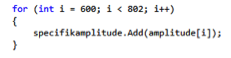
\includegraphics[width=0.6\textwidth]{Figurer/Snip20150525_44}
	\caption{Kode udsnit af analyse implementering}
\end{figure}

Disse værdier bliver derefter tjekket for, om de indeholder en amplitude, som ligger over tærskelværdien. Hvis dette er tilfældet, returnerer metoden ’true’, hvilket repræsenterer, at det er rigtigt, at denne patienten kan have atrieflimren. Hvis der ikke findes en værdi, som er højere end tærsklen, returnerer metoden ’false’, hvilket repræsenterer, at patienten ikke har atrieflimren. Dette kan ses på figur 6.7. 

\begin{figure}[H]
	\centering
	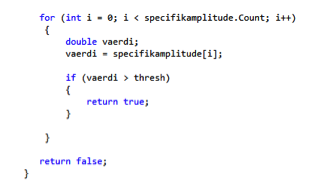
\includegraphics[width=0.8\textwidth]{Figurer/Snip20150525_47}
	\caption{Kode udsnit af analyse implementering}
\end{figure}

Tærskelværdien er blev fundet ud fra testprogrammet, som der kan læses yderligere om i dokumentationen 3.4.3. Der kan desuden også læses yderligere specifikation omkring implementeringen i dokumentationen 3.4. 


\subsection{Test}
I dette projekt er der hverken lavet modul eller integrationstest. I stedet er koden blevet testet efterhånden, som metoder er blevet færdiggjort. Det er også på denne måde, at gruppen har kunnet tjekke, at metoderne ikke melder fejl, eller får systemet til at bryde sammen. \\ \\
Metoden "KørEKG" kan give et eksempel på hvordan forløbet har været. "KørEKG" er en essentiel del af koden, og det var derfor vigtigt, at den fungerede fra starten af. Her blev den estimerede kode først skrevet, og derefter blev der kørt et EKG for at se, om grafen kom frem. Dette gjorde den ikke i første omgang, og der blev derfor tilføjet en linje kode, som henter den maksimale volt, som kommer igennem Analog Discovery, og det blev derefter en succes. \textbf{og hva så?? Virkede det så?}

\section{Resultater og diskussion}
Kravene til dette projekt er at afbilde, analysere og gemme EKG-signaler fra virtuelle patienter. Alt dette er lykkes. \\ 
Før det er muligt at starte en måling, skal man igennem et Login-vindue samt et CPR-vindue, hvor man indtaster den virtuelle patients CPR-nummer. Når login og CPR-nummeret til blevet godkendt vises EKG-vinduet, som er vinduet, hvor programmet køres fra. \\ \\
Ved tryk på "Start ny måling" går der X-antal sekunder og EKG-signalet bliver afbildet som en graf. Se figur 6.8. 

\begin{figure}[H]
	\centering
	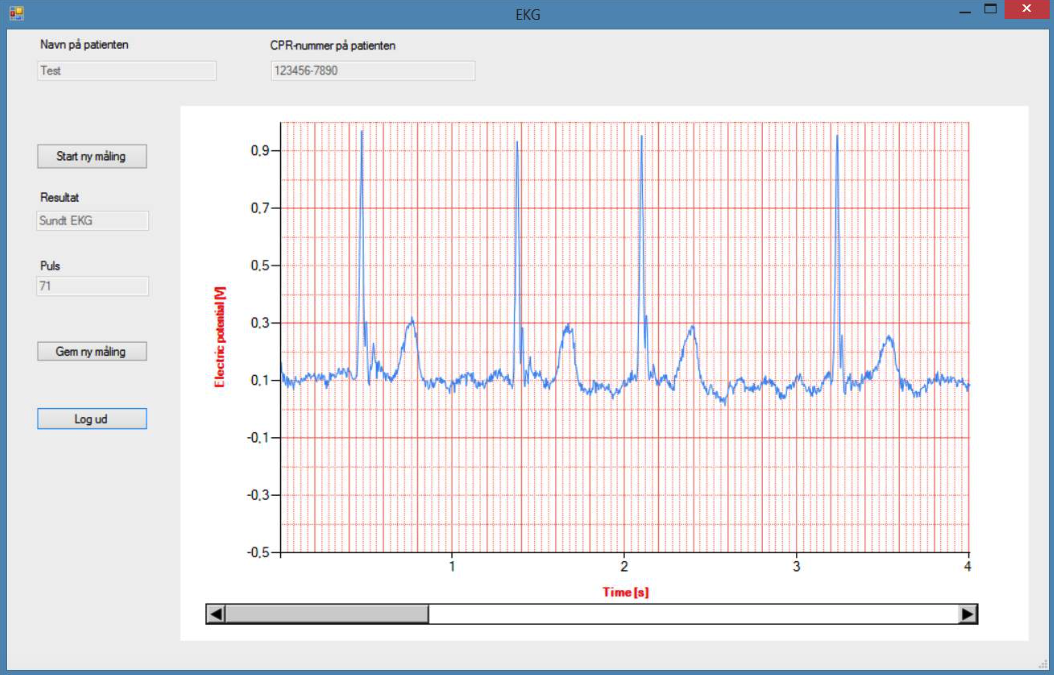
\includegraphics[width=1\textwidth]{Figurer/Snip20150525_25}
	\caption{Visning af EKG-signal samt analyse af sundt EKG-signal}
\end{figure}

Når EKG-grafen vises i EKG-vinduet har programmet også analyseret EKG-signalet i forhold til atrieflimren. Hvis EKG-signalet er normalt skriver programmet "Sundt EKG" under Resultat, se figur 6.8. Hvis EKG-signalet afviger fra standardværdierne (se under 3.2) skriver programmet "Tjek for Atrieflimmer!!", se figur 6.9. 

\begin{figure}[H]
	\centering
	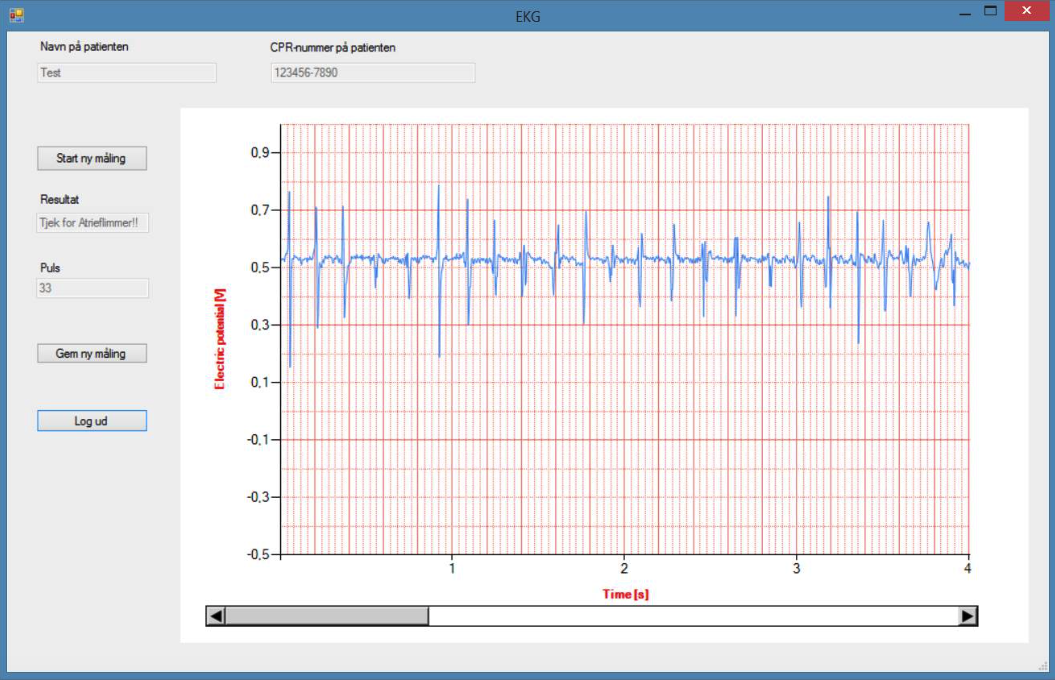
\includegraphics[width=1\textwidth]{Figurer/Snip20150525_26}
	\caption{Analyse af sygt EKG-signal}
\end{figure}

Efter visningen samt analysen af EKG-signalet skal målingens data gemmes i en privat- og offentlig database. Dette sker ved tryk på "Gem ny måling", hvorefter et pop-up vindue fremkommer og bekræfter handlingen. Efterfølgende kan man i den private database under "Måling"\--tabellen, se de gemte målinger, se figur 6.10.   

\begin{figure}[H]
	\centering
	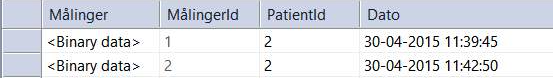
\includegraphics[width=1\textwidth]{Figurer/Snip20150525_27}	
	\caption{Lagring af data i privat database}
\end{figure}

I den offentlige database er der to tabeller. Den ene hedder EKG\_Data, hvor den virtuelle patients og brugerens data gemmes, se figur 6.11. Den anden hedder EKG\_måling, hvor informationer omkring selve målingen gemmes, se figur 6.12. 

\begin{figure}[H]
	\centering
	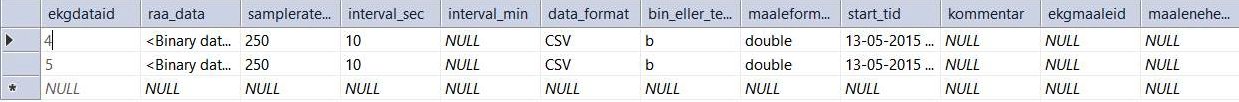
\includegraphics[width=1\textwidth]{Figurer/Snip20150525_28}
	\caption{Lagring af den virtuelle patients- og brugerens data i den offentlig database}
\end{figure}

\begin{figure}[H]
	\centering
	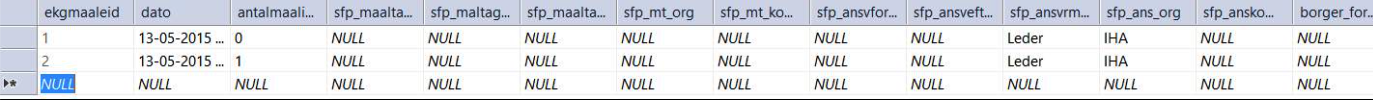
\includegraphics[width=1\textwidth]{Figurer/Snip20150525_29}
	\caption{Lagring af målingens data i offentlig database}
\end{figure}

Med hensyn til visningen af målingen, kunne der godt have været et mere præcis gitter, således at brugeren nemmere kunne aflæse ud fra grafen om patienten har atrieflimren. Det kan godt lade sig gøre at aflæse på nuværende tidspunkt, men det er mindre præcis, da ternene ikke er kvadratiske.

Det har ikke været muligt at gøre analysen så præcis, at den kunne detektere atrieflimren helt præcist, men derimod gør den brugeren opmærksom på, at der er en anormalitet i forhold til et normalt EKG-signal. Analysen kunne ikke gøres præcis, da der findes mange forskellige typer af EKG-signaler, der repræsenterer atrieflimren, som følge af, at mennesker er forskellige.

Da det kom sent ud, at der skulle kunne gemmes i en offentlig database, er flere af værdierne blev fravalgt pga. tidspres. Dog kunne der have været indskrevet nogle flere værdier, således at f.eks. patientens CPR-nummer og navn kunne lægges ind og gemmes i tabellen EKG\_Data.

I kapitel 4 i dokumentationen kan resultatet af accepttesten læses. 


\section{Opnået erfaringer}

VI SKAL HAVE NOGET OM HVAD GRUPPEN TILSAMMEN HAR OPNÅET - BARE KORT. 


\textbf{Lise Skytte Brodersen}\\

\textbf{Mads Fryland Jørgensen}\\

\textbf{Albert Jakob Fredshavn}\\
I dette projektet har jeg arbejdet med projektdokumentationen. Til at arbejde med dette har vores del af projektgruppen benyttet de redskaber som blev undervist i, i ISE lektionerne, samt dele af vores anatomi og fysiologi undervisning. De modeller og metoder som blev taget i brug var meget overensstemmende med det som vi havde lært og gav en god relation til det arbejde vi skulle igennem. Vi blev delt i to undergrupper gennem projekt, en der stod for programmeringen og en der stod for dokumentationen gennem projektet. Denne opdeling og uddelegering gjorde at den ene gruppe ikke havde særlig stor indflydelse på hvad den anden gruppe lavede, i henhold til at følge processen gennem projektet. Det er dog blevet gennemgået ned til detaljer og beskrevet i selve kode-delen af programmet med udkommenterede linjer tekst. \\
Projektarbejdet i gruppen har forgået ganske godt. Der blev fra start til slut holdt regelmæssige gruppermøder med vores projektvejleder. Dette har klart været en fordel da det har forventningsafstemt vores forskellige opgaver gennem projektet. Samtidig har gruppen, i nogen omfang, været god til at kommunikerer med hensyn til hvor langt de enkelte var, og med hvad. Stemningen i gruppen har været ambitiøs uden at man følte et tungt pres på skuldrene. Ligeledes har stemningen været afslappet nok til at man kunne stille spørgsmål og få hjælp til diverse opgaver igennem projektets forløb.\\

\textbf{Malene Cecilie Mikkelsen}\\
Da vi startede projektet, delte vi gruppen op i to grupper, hvilket vi følte var en nødvendighed for at kunne nå det hele. Desværre havde det den følgevirkning, at kommunikationen mellem de to grupper blev lidt halvhjertet, således at der af flere omgange blev brug for at lave ændringer, og der var nogle enkelte diskussioner mellem grupperne. I gruppen var det aftalt ikke at have en leder, men jeg synes ikke, at det fungerer ordentlig, da der mangler en, som har noget overblik. Heldigvis tog Lise styringen i løbet af projektet, dog havde det været en fordel, hvis dette havde været klart fra starten. 
Selve emnet har været meget relevant, og det har givet en del erfaring til arbejdsmarkedet. Særligt den ekstra del med den ekstra database, som kom ud, da vi efterhånden troede, at vi var færdig, pressede gruppen en del, men gav en erfaring med, at det er sådan noget, som man kan komme ud for senere på arbejdsmarkedet.
Projektet er blevet fuldført, men jeg synes, at vi kun lige har fuldført den. Vi havde mange gode ideer, da vi startede, men det mundede ud i, at vi kun fik lavede det mest nødvendige. Til næste projekt kunne jeg godt tænke mig, da der blev arbejdet lidt mere fokuseret, og at der blev stillet lidt højere krav indenfor gruppen.

\textbf{Mohammed Hussein Mohamed}\\

\textbf{Sara-Sofie Staub Kirkeby}\\
I dette projekt, har jeg primært arbejdet med det programmeringsmæssige aspekt. Personligt, syntes jeg det har været en anelse frustrerende, da der i den sammenhæng, er dukket nogen ting op, som ikke har været en del af vores undervisning, i dette semester. Det har krævet meget tænkning ud af boksen. Dette har selvfølgeligt også gjort, at vi har været tvunget til, at lære os selv, yderligere ting. \\
Jeg har siddet med det overordnede ansvar for analysen, og det viste sig at være mere problematisk, end først regnet. Analysen blev ændret tre gange undervejs, og hver eneste gang, har der været behov for, at skrive analysen fuldstændig om. Her har vejleder dog været rigtigt god til, at træde til, og give et andet syn på, hvordan analysen kunne laves, og det hjalp meget.\\ 
Et andet problem har været, at vi valgte at dele gruppen op i to; en der lavede det meste tekstarbejde, og en anden del, som stod for programmeringen. Kommunikationen imellem de to undergrupper, har til tider ikke været særligt godt, og det har betydet at vi er blevet nødt til at ændre nogen ting undervejs. \\
Jeg mener generelt at jeg har lagt et godt stykke arbejde i gruppen, og jeg har forsøgt at gøre så meget jeg overhovedet kunne. Jeg har lært meget om EKG-signaler og deres karakteristikker, samt omkring, hvordan sådan et program skal programmeres. Jeg kunne dog eventuelt godt have forsøgt at tage mere initiativ, og have taget lidt mere kontakt med skriveholdet. \\
Projektet er efter min mening gået rigtigt godt, og jeg mener at det er et stykke arbejde vi godt kan være stolte af.

\textbf{Martin Banasik}\\
I dette 2. semesterprojekt som omhandler måling af EKG, har jeg været med til at programmere vores program fra start til slut. Dette har omfattet vores første overvejelser hvordan vores program skulle se ud og hvilke funktioner det skulle have, til et færdig program som jeg er godt tilfreds med. I forprojektet fandt jeg det svært at komme i gang med og forstå hvad det skulle kunne, men efterhånden jeg man satte sig mere ind i koden, hjalp det på forståelsen og kunne gøre brug af og overføre de ting jeg havde lært i programmering til vores eget projekt og program. Det har øget min interesse for programmering og finder det spændende at lave et program fra bunden, ud fra fordefineret krav og funktion. 

Jeg synes at samarbejdet har været fint og har fungeret i programmerings gruppen. Selvom at vi i starten var i tvivl om hvordan vi skulle gribe det hele an og samtidigt med at vi alle havde vores egne ideer til hvordan det skulle være, synes jeg at vi er kommet frem til et resultat, hvor alle har haft deres indflydelse. Der var ideer som vi gerne ville have med i programmet, men efter evne og deadlines blev droppet, hvilket man kunne til en anden gang have mere fokus på, så disse blev en realitet. 

\textbf{Cecilie Ammitzbøll Aarøe}\\
Igennem dette projekt arbejdede jeg i den gruppe som bla. udarbejdede projektdokumentationen. Det gjorde at jeg fik mulighed for at arbejde med nogle af de værktøjer, som vi har lært i ISE. En ulempe har dog været, at jeg dermed ikke var med til at programmere programmet. Den del af gruppen, som programmerede, var dog meget gode til at udkommantere programmering, så vi andre nemt kunne sætte os ind i den. Desuden afholdte vi enkelte møde, hvor programmeringen blev gennemgået i de mindste detaljer. Men det er stadigvæk ikke det samme som at sidde med det selv.\\
Jeg synes gruppen har arbejdet godt sammen, og vi havde fra starten afstemt vores forventninger til projektet. At disse forventninger så var lidt højere end det var muligt at efterkomme, er noget der altid vil ske i starten af et projekt. Men jeg vil hellere hav store forventninger til et projekt og så afstemme dem med hvad der er realistisk, frem for at sætte baren lavt fra starten.\\
Vi havde også lidt kommunikations vanskeligheder i starten af projektet. Dokumentationsgruppen skulle designe systemet udfra funktionelle og ikke-funktionelle krav. Vi rådførte os med programmeringsgruppen, men der opstod en misforståelse mellem grupperne, som gjorde at vi ikke helt havde forstået hvad systemet helt præcist gjorde.\\
Men alt i alt synes jeg, det har været en god oplevelse at lave dette projekt. Gruppen har fungeret rigtig godt. Der har været en god stemning, og vi har været gode til at hjælpe hinanden, når der var brug for det.

\section{Fremtidigt arbejde}
Som følge af at projektet er tiltænkt som en prototype, er der løbende gennem projektudførelsen opstået en masse muligheder og idéer for videreudvikling af systemet. \\\\
Den første helt basale idé, som også er forsøgt udført sideløbende i projektet, er etablering af en "opret ny patient"\--funktion. Funktionen skal muliggøre, at brugeren kan oprette en ny patient i systemet, i forbindelse med indtastning af patientens CPR-nummer. Funktionen skal fungere således, at hvis ikke det indtastede CPR-nummer i forvejen er kendt i systemet, skal skridtet efter CPR-vinduet være et nyt "Opret Patient"\--vindue. Her skal brugeren kunne indtaste relevante oplysninger omkring patienten, og til slut oprette patienten i både den private- og offentlige database.\\\\
Et ideelt område til videreudvikling er brugervenlighed, både på software plan og i særhed på hardware plan.\\
Software kan udvikles i en retning, hvor det bliver lettere og mere overskueligt for brugeren, at analysere og evaluere EKG-signalet. En forbedring ville være, at der skal være mulighed for at trække en eller flere x- og y-cursors ned over EKG-signalet, og dermed få vist amplitude, tid og relevante intervaller. Herefter kunne en mulighed være, at de observerede værdier kunne gemmes som tilhørende tekst til det specifikke EKG-signal. \\
Sideløbende, imens EKG-målingen foretages, vil det være muligt, at have direkte adgang til den pågældende patients sygejournal. Adgangen til sygejournalen skal kunne læses i en et andet vindue, som er synligt samtidig med EKG-vinduet arbejder, hvorefter det er muligt at skifte mellem disse vinduer, og tilføje ændringer, notater etc. i journalen. Med andre ord skal systemet understøtte EPJ.\\ \\
Den endelige udgave af softwaren skal implementeres på et mere brugervenligt interface, eksempelvis en tablet eller lignende. Samtidig kan systemet være tilknyttet en håndholdt EKG-måler, i form af en holter, hvorefter softwaren aflæser data, og udskriver på tabletten.\\ Desuden skal det være muligt for brugeren at vælge indstillinger alt efter, hvad der ønskes analyseres for. Prototypen er kun tilpasset analyse for atrieflimren, men med det endelige produkt skal være muligt at kunne vælge undersøgelse for eksempelvis andre hjertesygdomme. De forskellige undersøgelser skal derudover også kunne mixes på kryds og tværs, hvis patienten har blandede symptomer, således at der søges for flere sygdomme. Dette vil medføre, at brugeren kan tage udstyr med sig på hjemmebesøg, såvel som at patienten selv kan foretage en måling.

